\chapter*{Objetivo}
El objetivo de este manual es proporcionar los pasos precisos para hacer uso del aplicativo web de Distrifulll.

\begin{definicion}
	{\rm \url{https://distrifull.herokuapp.com/}: } el aplicativo de Distrifulll, es un aplicaci\'on que facilita el monitoreo de los tanques de almacenamientos de aceites industriales, proporcionando en tiempo real la capacidad de almacenamiento, el costo general. 
\end{definicion}

\chapter*{Desarrollo del manual de usuario}

\section*{\'Area principal}

\begin{figure}[h!]
	\centering
	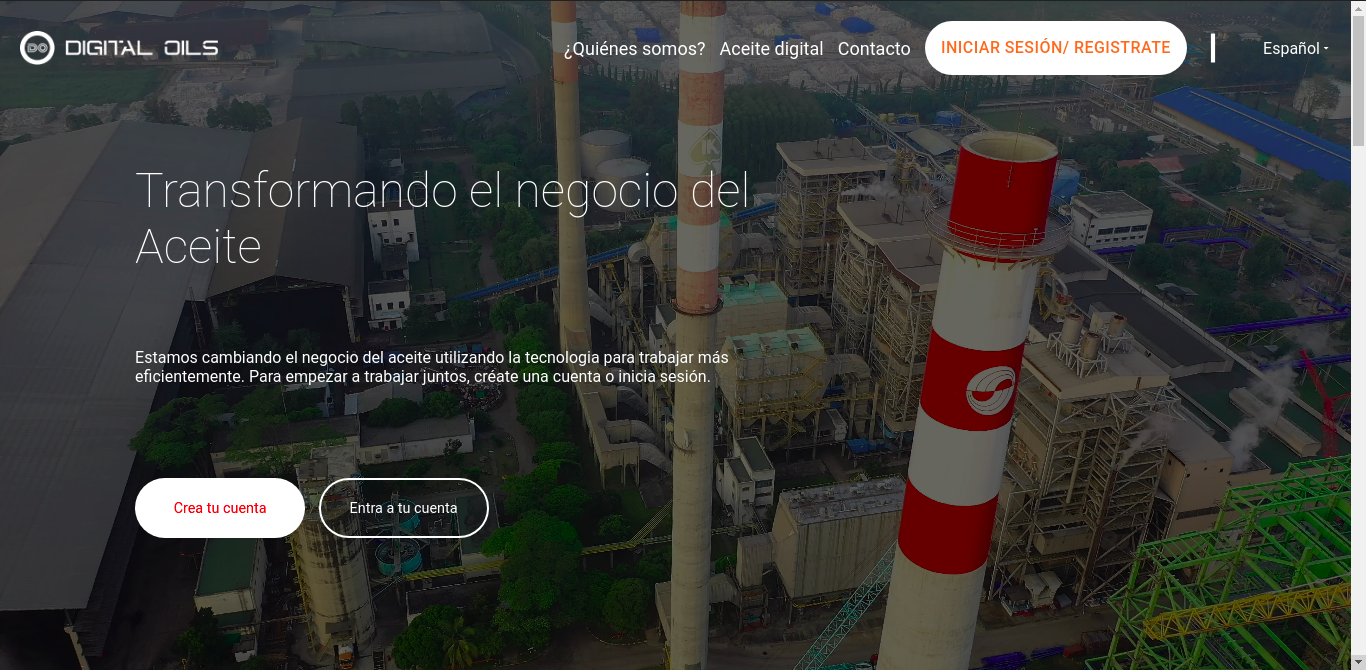
\includegraphics[width=1\linewidth, height=0.4\textheight]{imagenes/inicioOne}
	\caption[Primera parte del inicio.]{}
	\label{fig:inicioone}
\end{figure}
Esta secci\'on encontramos en la parte superior izquierda el logo de la empresa y en la parte derecha encontramos acceso directo a las secciones visibles a todo tipo de usuario, entre ellas tenemos:
\begin{enumerate}
	\item ?` Qui\'enes somos?
	\item Aceite digital.
	\item Iniciar sesi\'on y registrarse.
	\item Idioma.
\end{enumerate}

\subsection*{?`Qui\'enes somos?}

%\begin{figure}[h!]
%	\centering
%	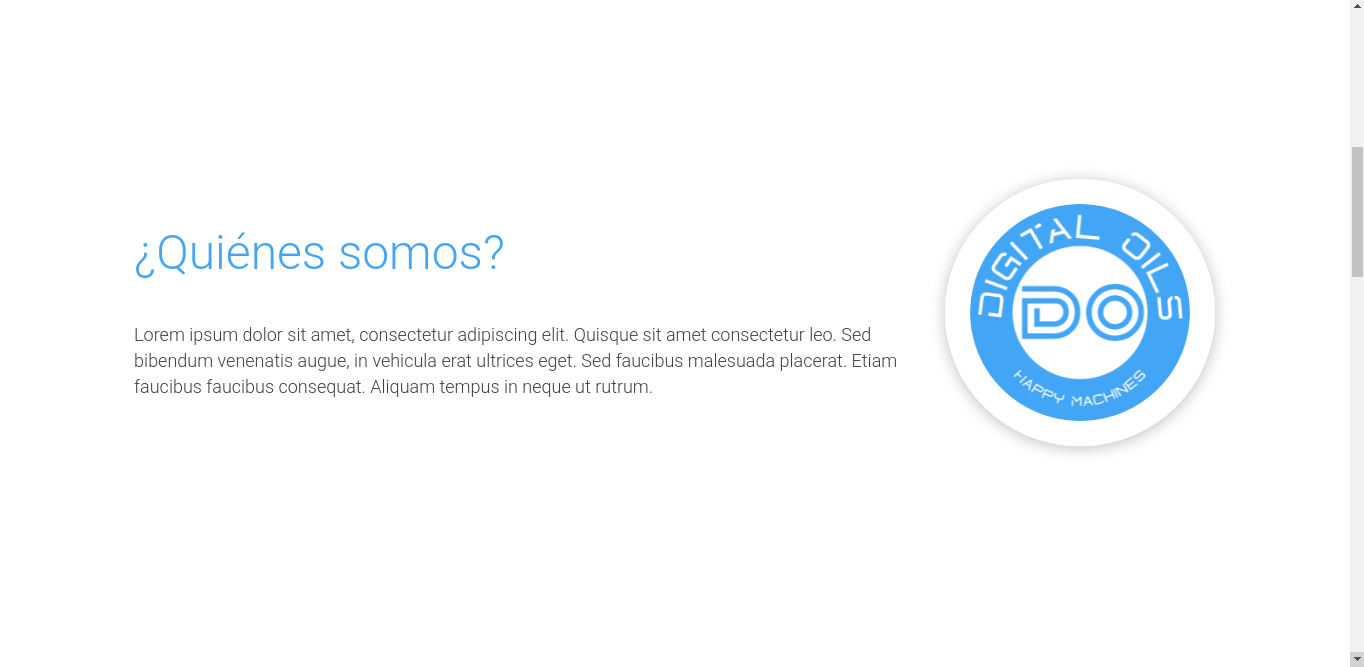
\includegraphics[width=1\linewidth, height=0.4\textheight]{imagenes/inicioTwo}
%	\caption[`?Qui\'enes somos?.]{}
%	\label{fig:inicioTwo}
%\end{figure}

En esta secci\'on encontramos un breve explicaci\'on sobre la empresa.

\subsection*{Aceite d\'igital}

\begin{figure}[h!]
	\centering
	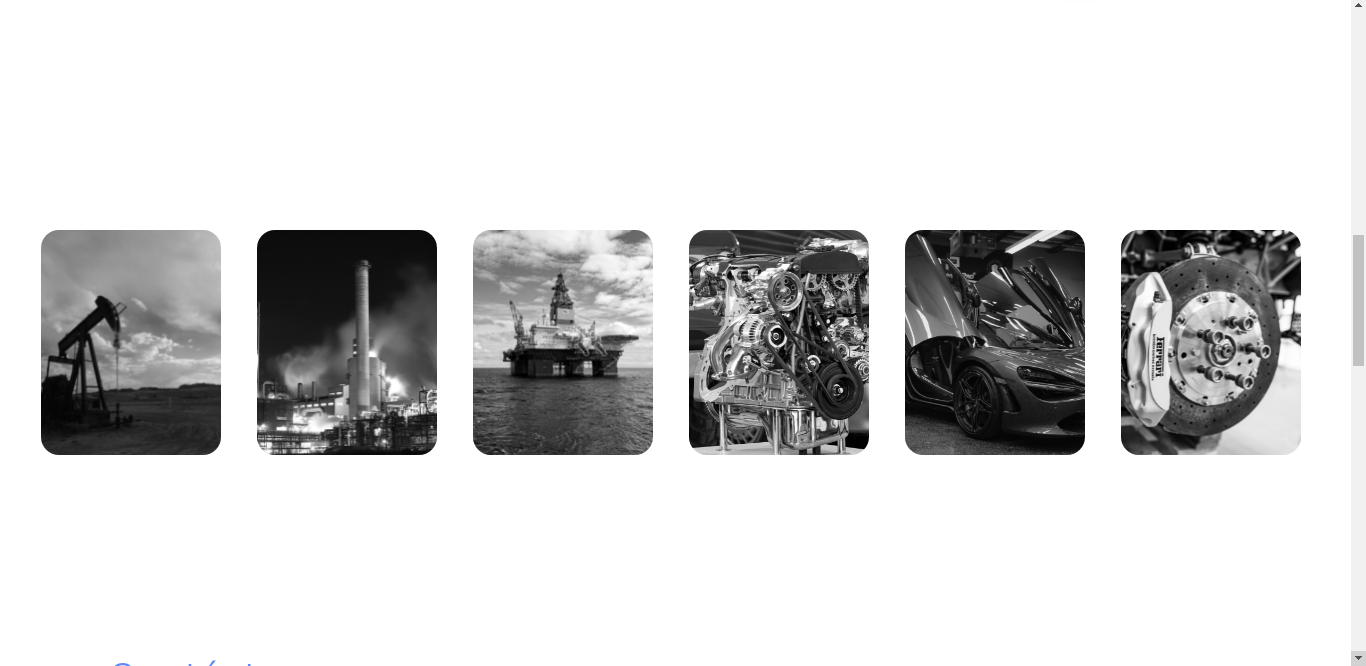
\includegraphics[width=1\linewidth, height=0.4\textheight]{imagenes/inicioThree}
	\caption[Tercera  parte del inicio.]{}
	\label{fig:inicioThree}
\end{figure}
En esta secci\'on encontramos una serie de productos ofrecidos por la empresa.

\begin{figure}[!]
	\centering
	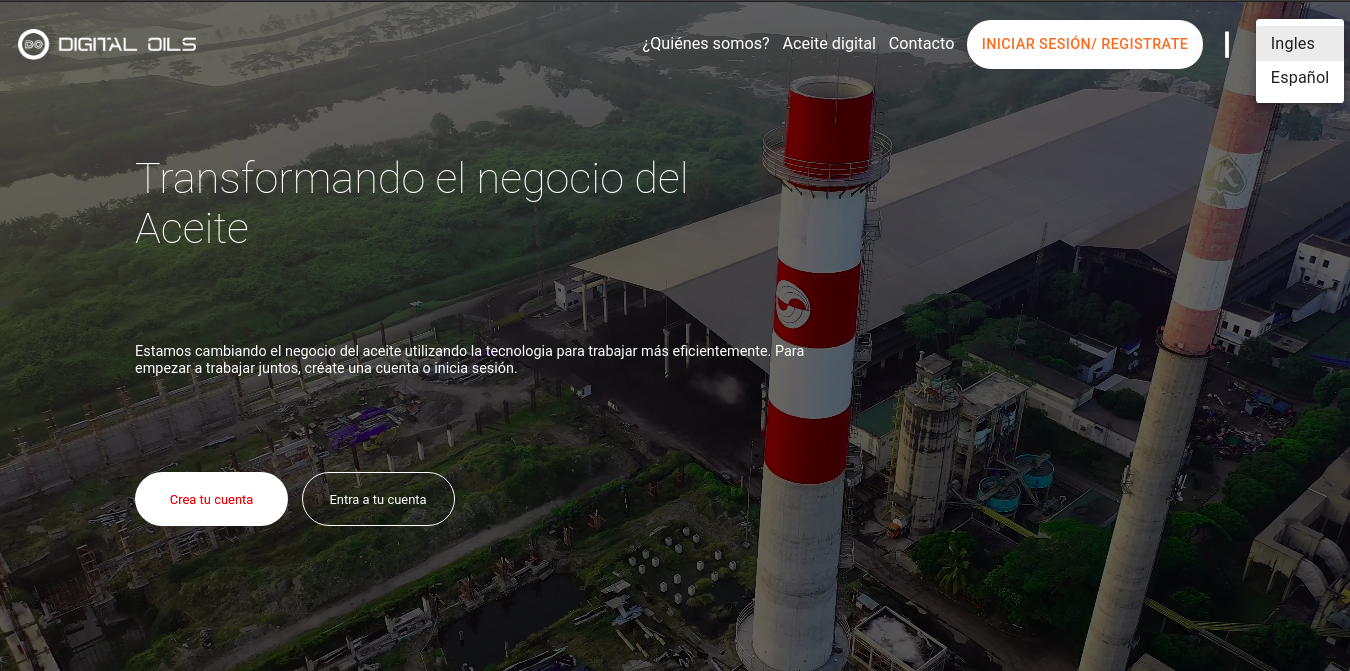
\includegraphics[width=1\linewidth, height=0.4\textheight]{imagenes/inicioOneIdioma}
	\caption[\'Area principal.]{}
	\label{fig:iniciooneidioma}
\end{figure}



\begin{figure}[!]
	\centering
	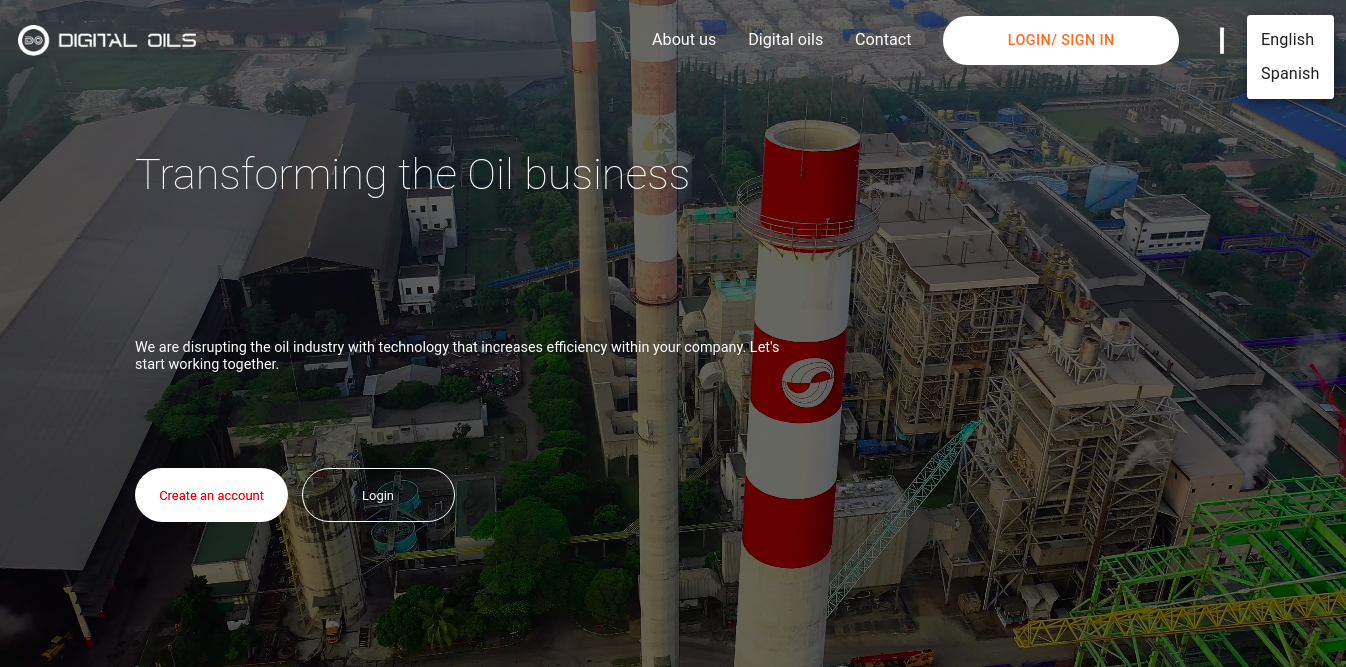
\includegraphics[width=1\linewidth, height=0.4\textheight]{imagenes/inicioOneIngles}
	\caption[Primera parte del inicio.]{}
	\label{fig:iniciooneingles}
\end{figure}


\begin{figure}[!]
	\centering
	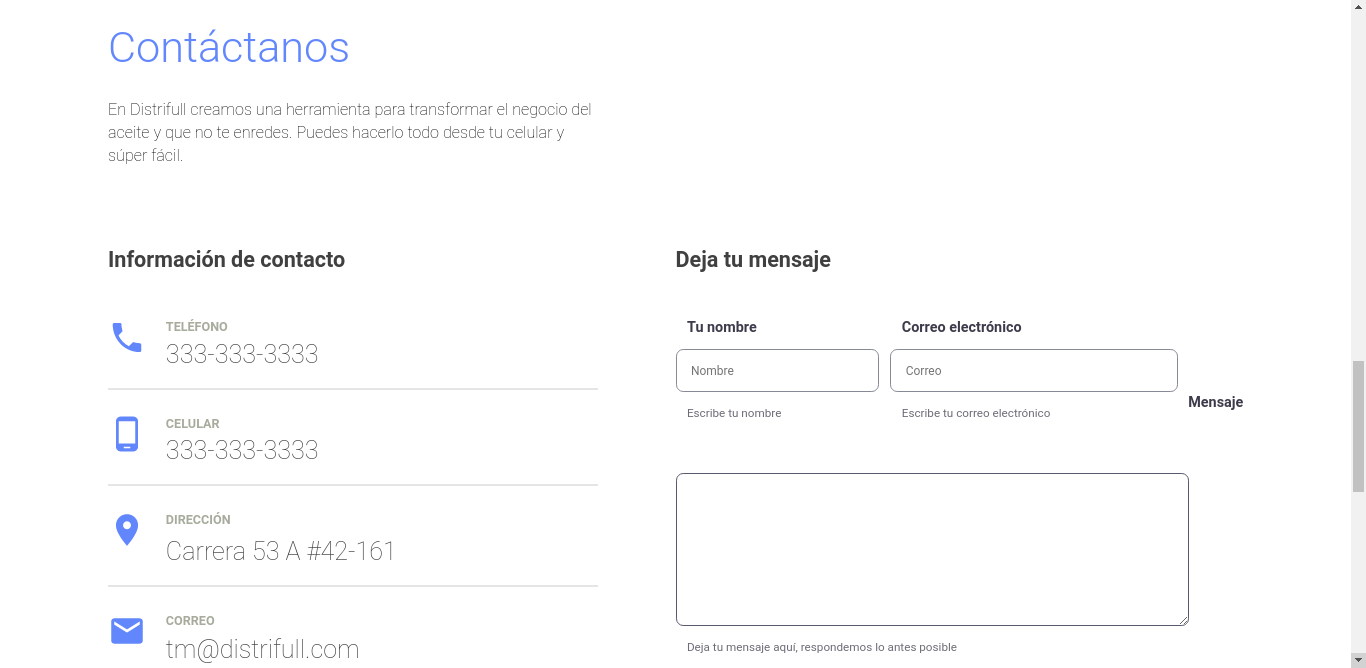
\includegraphics[width=1\linewidth, height=0.4\textheight]{imagenes/inicioFour}
	\caption[Cuarta parte del inicio.]{}
	\label{fig:inicioFour}
\end{figure}

\begin{figure}[!]
	\centering
	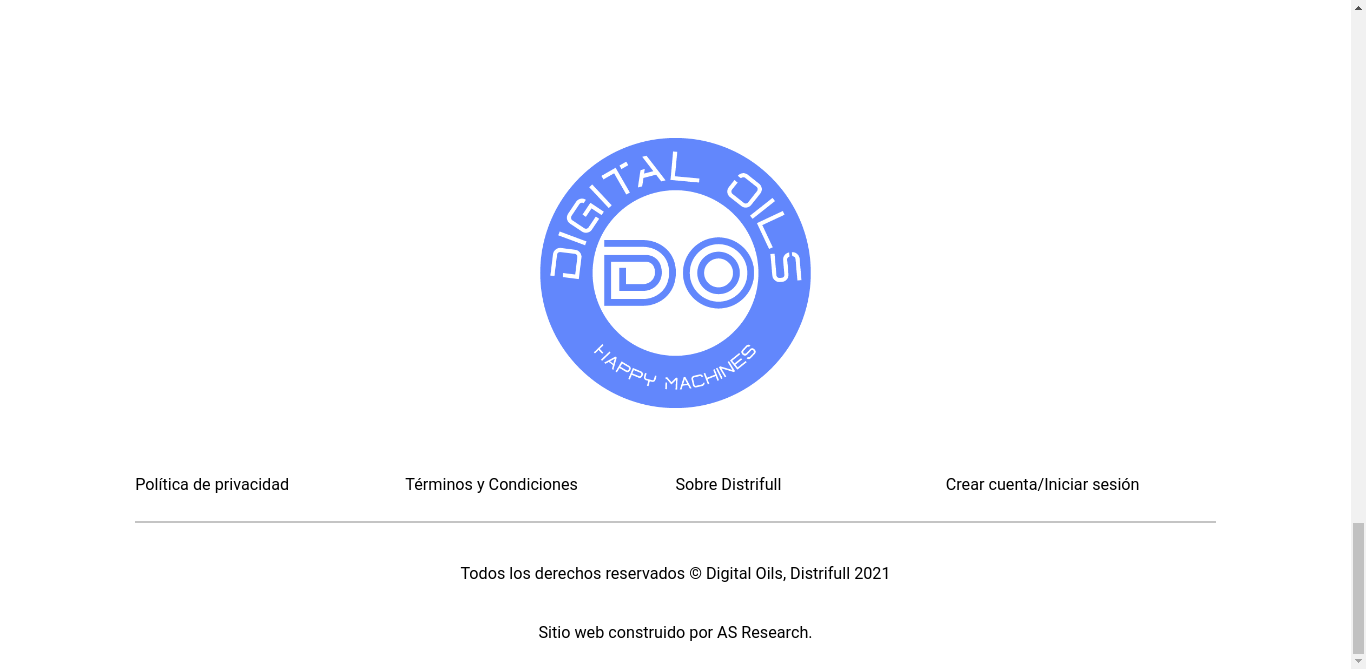
\includegraphics[width=1\linewidth, height=0.4\textheight]{imagenes/inicioFive}
	\caption[Quinta parte del inicio.]{}
	\label{fig:inicioFive}
\end{figure}

\begin{figure}[!]
	\centering
	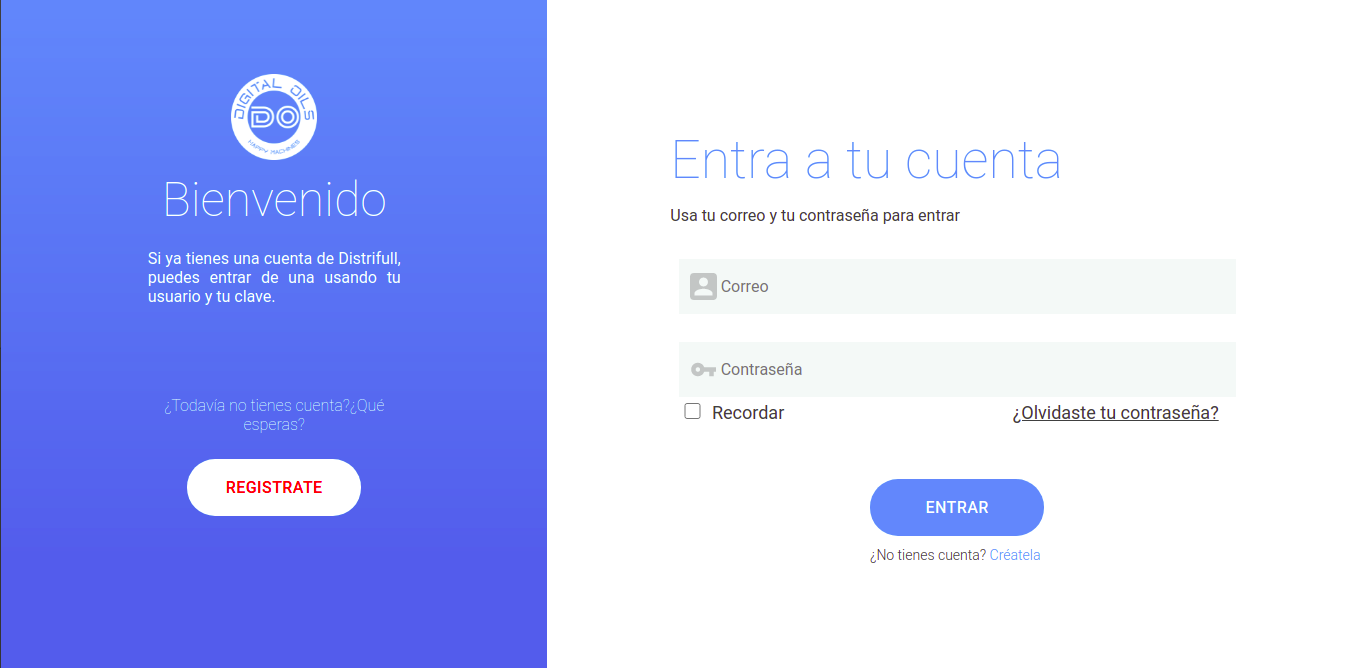
\includegraphics[width=1\linewidth, height=0.4\textheight]{imagenes/inicioSesion}
	\caption[Inicio de sesi\'on.]{}
	\label{fig:iniciosesion}
\end{figure}

\begin{figure}[!]
	\centering
	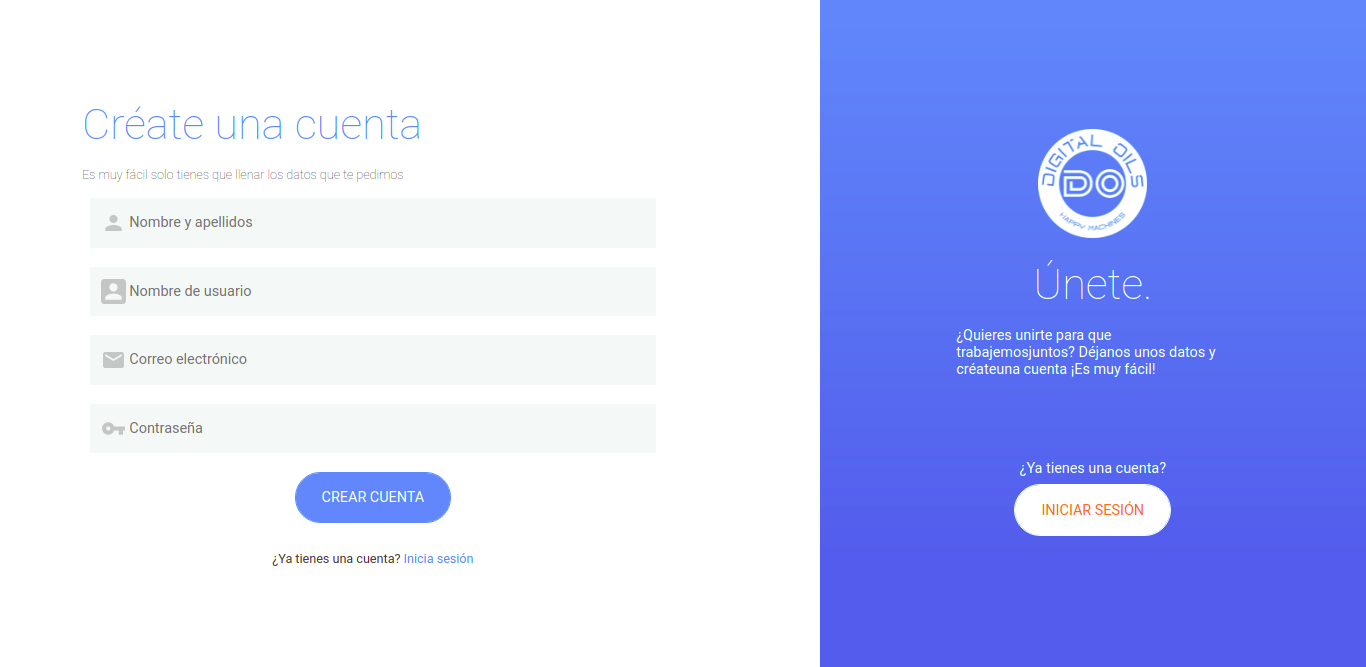
\includegraphics[width=1\linewidth, height=0.4\textheight]{imagenes/registro}
	\caption[Registro de sesi\'on.]{}
	\label{fig:registro}
\end{figure}

\section{Parte interna para los usuarios}
En las siguientes sesiones cobra mucha importancia el rol del usuario, ya que este le permite ver cierto contenido del aplicativo web. 

\begin{figure}[h!]
	\centering
	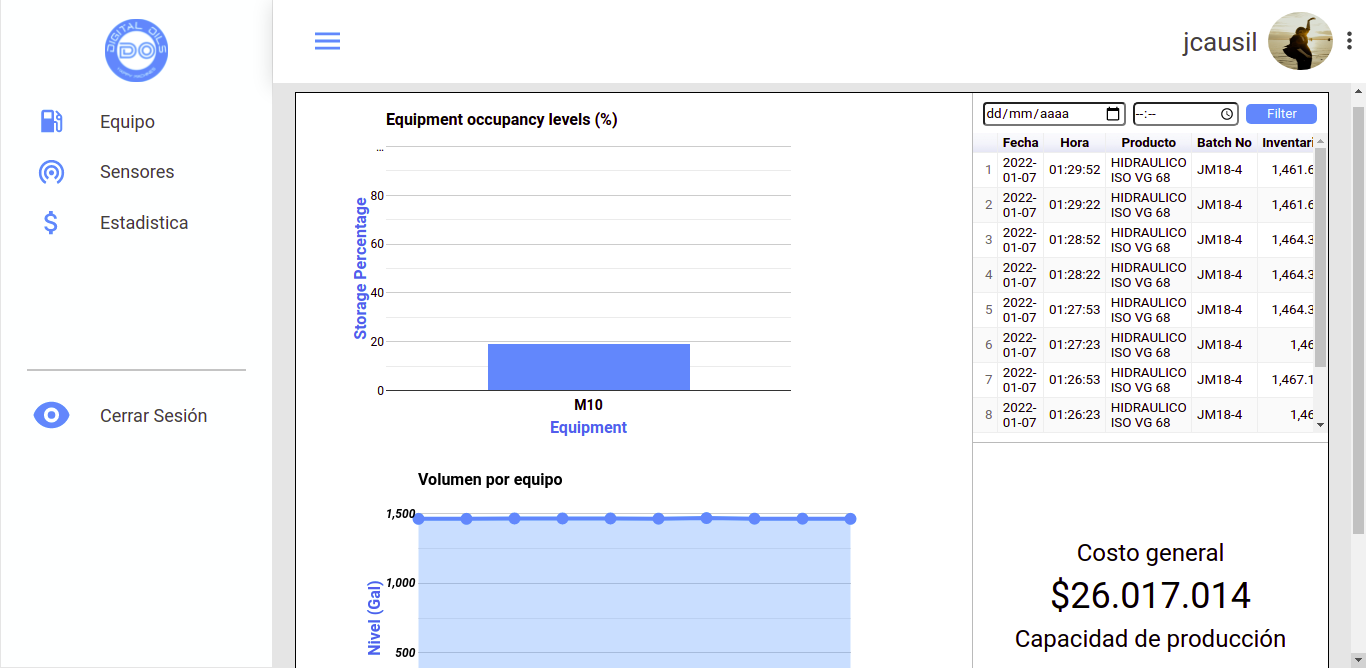
\includegraphics[width=1\linewidth, height=0.4\textheight]{imagenes/dashboardAdmi}
	\caption[Primera parte del inicio.]{}
	\label{fig:dashboardAdmi}
\end{figure}



\begin{figure}[!]
	\centering
	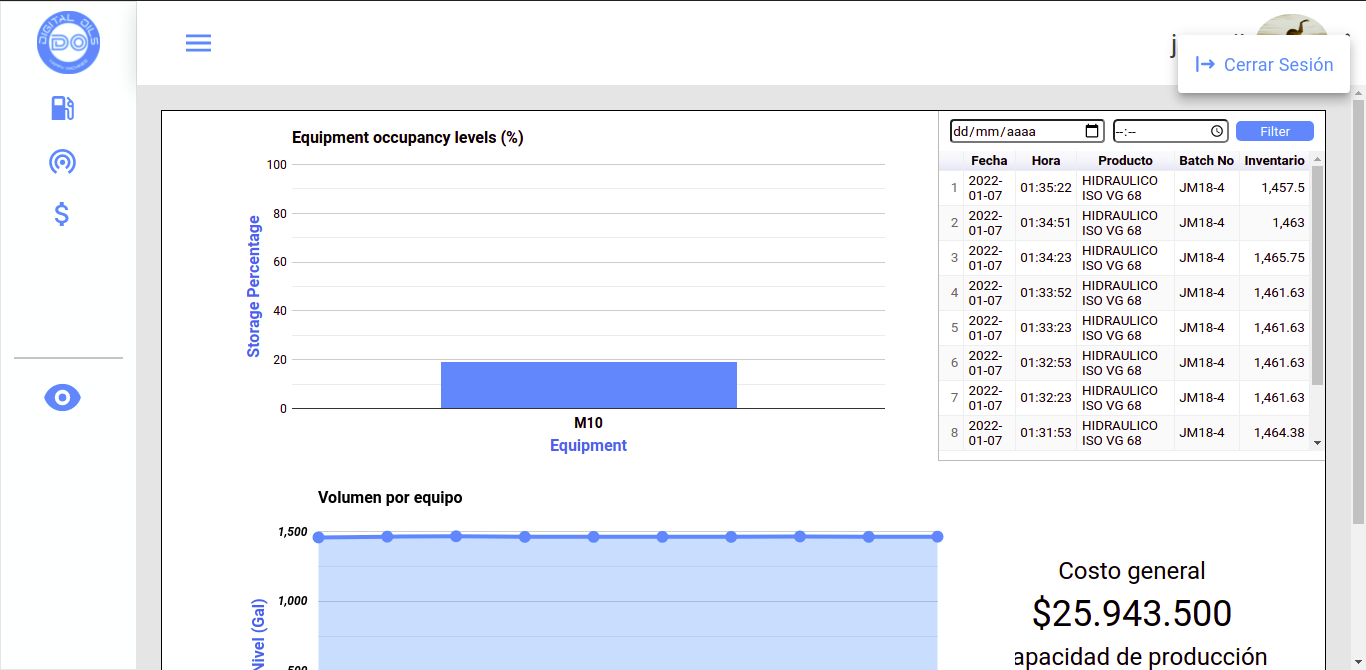
\includegraphics[width=1\linewidth, height=0.4\textheight]{imagenes/dashboardExit}
	\caption[Primera parte del inicio.]{}
	\label{fig:exitDashboard}
\end{figure}

\begin{figure}[!]
	\centering
	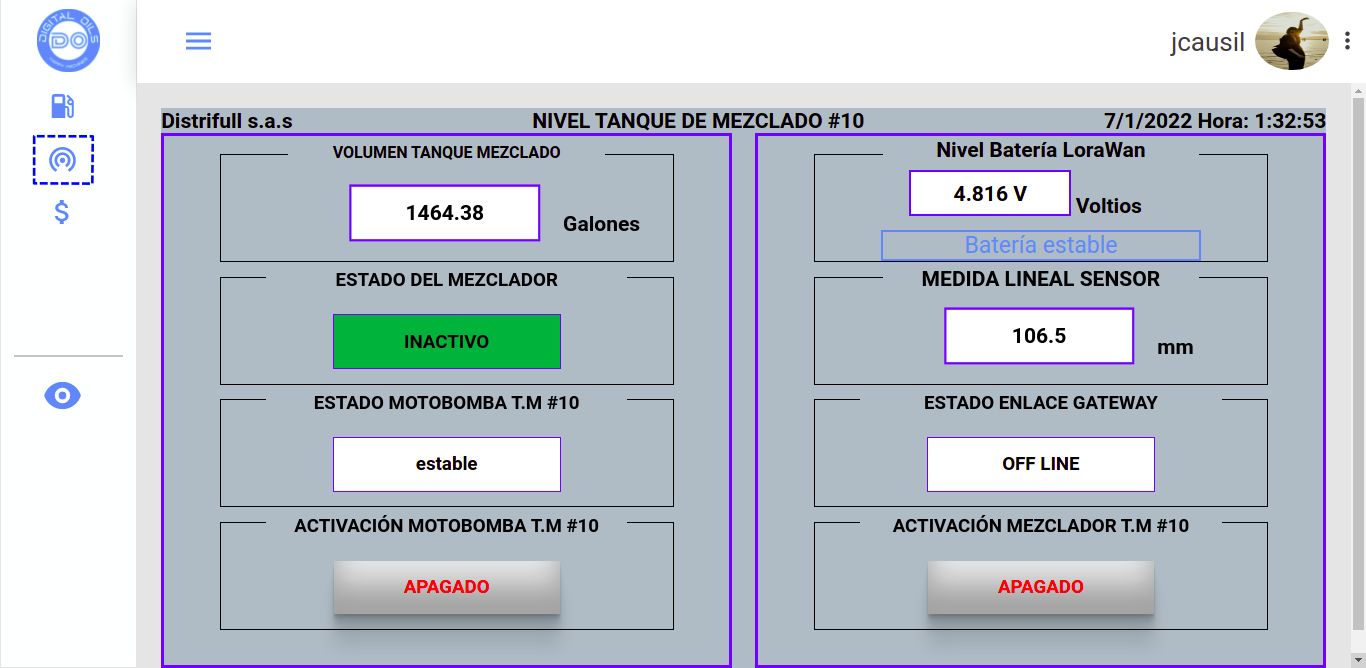
\includegraphics[width=1\linewidth, height=0.4\textheight]{imagenes/dashboardSensores}
	\caption[Primera parte del inicio.]{}
	\label{fig:dashboardSensores}
\end{figure}

\begin{figure}[!]
	\centering
	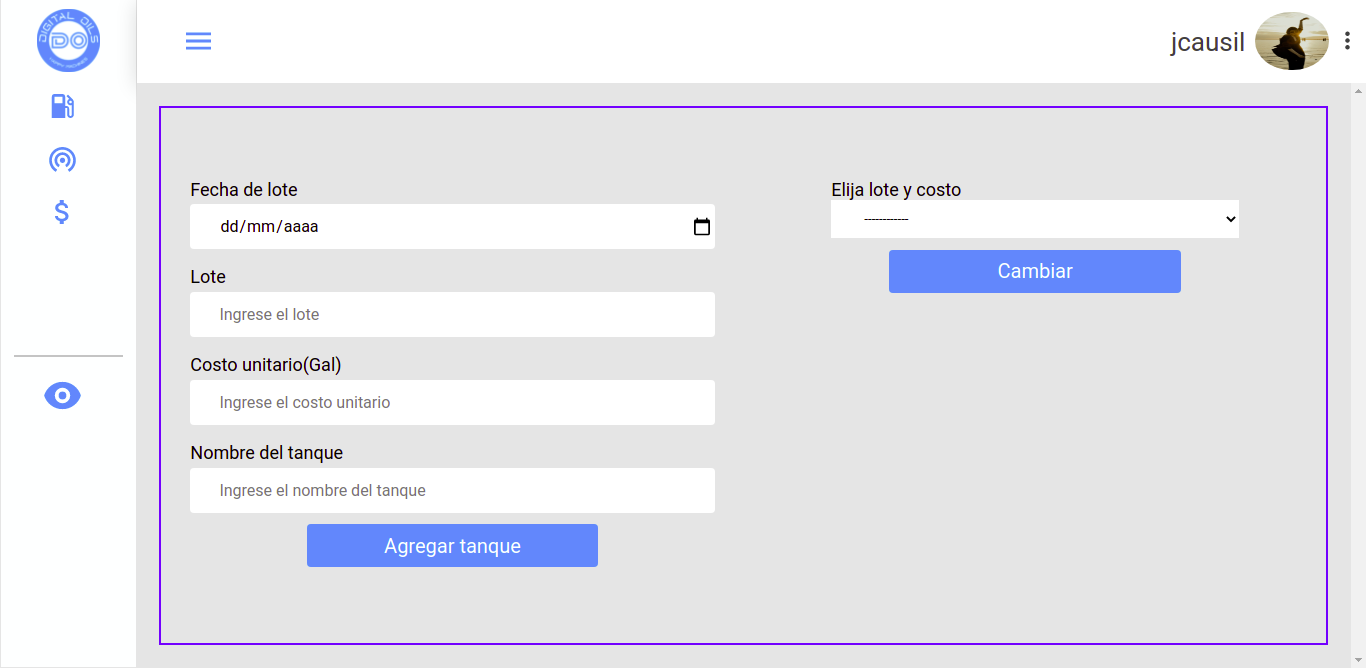
\includegraphics[width=1\linewidth, height=0.4\textheight]{imagenes/dashboardEstadistica}
	\caption[Primera parte del inicio.]{}
	\label{fig:dashboardEstadistica}
\end{figure}